\documentclass{article}

\usepackage{graphicx}
\usepackage{fancyhdr}
\usepackage[sorting=none]{biblatex}
\usepackage[margin=1in, top=1in]{geometry}
\usepackage{listings}
\usepackage[hidelinks]{hyperref}
\usepackage{xcolor}
\usepackage{xepersian}

\addbibresource{bibliography.bib}
\settextfont[Scale=1.3]{B-NAZANIN.TTF}
\setlatintextfont[Scale=1]{DejaVuSans}
\renewcommand{\baselinestretch}{1.5}
\pagestyle{fancy}
\fancyhf{}
\rhead{درخت تصمیم}
\lhead{مهلت تحویل پروژه: ۱۴ اردیبهشت ۱۴۰۳}
%\rfoot{مبنا های عددی}
%\lfoot{9700000}
\renewcommand{\headrulewidth}{1pt}
\renewcommand{\footrulewidth}{1pt}



\begin{document}
	\begin{centering}
		\LARGE
		پروژه دوم مبانی هوش محاسباتی \\
	\end{centering}
	\section*{مقدمه}
	دیتاستی مرتبط با ماشین ها در اختیار شما قرار گرفته است؛ دیتاست فوق به دو بخش \lr{train} و \lr{test} تقسیم شده است. در این پروژه از شما می‌خواهیم تا درخت‌تصمیمی بسازید، که بتواند داده های آموزشی را بر اساس مدل ماشین، طبقه‌بندی کند؛ سپس از دیتای \lr{test} برای ارزیابی عملکرد مدل خود استفاده کنید. درخت تصمیم ساخته شده، باید منطبق بر موارد تدریس شده در کلاس باشد.
	
	\section{فاز اول}
	این دیتاست، شامل تعدادی \lr{Missing data} می‌باشد. با توجه به روش های مطرح شده در کلاس درس، می‌بایست این مورد را هندل کنید. نتایج حاصل از هر کدام از روش ها را بررسی و تحلیل نمائید؛ همچنین نتایج را با هم مقایسه کنید.
	\\
	دراین بخش برای \lr{load} کردن و پردازش دیتا، می‌توانید از کتابخانه \lr{\href{https://pandas.pydata.org/}{\textcolor{blue}{Pandas}}} استفاده نمائید. 
	
	\section {فاز دوم}
	همانطور که در درس خوانده اید، از الگوریتم \lr{ID3} برای ساخت درخت تصمیم استفاده می‌شود؛ با استفاده از این الگوریتم درخت تصمیم مناسبی بسازید که با محاسبه \lr{Entropy} و \lr{Information Gain} در هر مرحله \lr{Attribute} مناسب را انتخاب کند. برای این منظور نیاز به پیاده‌سازی کلاس \lr{Node} دارید؛ همچنین توابع  \lr{Entropy} و \lr{Information Gain} را نیز خودتان باید پیاده سازی کنید. در این فاز موارد زیر را بررسی و گزارش کنید.
	\begin{itemize}
		\item [$\bullet$] نحوه تشکیل درخت و انتخاب فیچرها را به طور کامل بررسی کنید.
		\item [$\bullet$] راه حل خود را برای فیچرهای پیوسته توضیح دهید (دقت داشته باشید که باید مقدار بهینه  \lr{Threshold} را برای گسسته سازی این نوع فیچر ها استفاده نمائید).
		
		\item [$\bullet$] بررسی کنید که چه زمانی \lr{Entropy} و \lr{Information Gain} به مقدار حداکثر خود می‌رسند.
	\end{itemize}
	
	\section{فاز سوم}
	یکی از مشکلات درخت تصمیم، \lr{Overfit} شدن آن است؛ بررسی کنید که این مشکل چه زمانی به وجود می‌آید و برای حل این مشکل حداقل دو راه حل را بررسی نمائید (نیازی به پیاده سازی نیست).
	
	\section{فاز چهارم}
	در نهایت درخت ساخته شده را \lr{visualize} کنید (مشابه شکل ۱). در هر \lr{Node} درخت، نام \lr{Attribute} ها،  \lr{Entropy} و \lr{Information Gain} مربوطه را ذکر کنید. برای این منظور می‌توانید از کتابخانه  هایی مانند \lr{\href{http://www.graphviz.org/}{\textcolor{blue}{Graphviz}}}، \lr{\href{https://plotly.com/}{\textcolor{blue}{Plotly}}}  و یا ابزار های مشابه استفاده نمائید.
	\begin{figure}
		\centerline{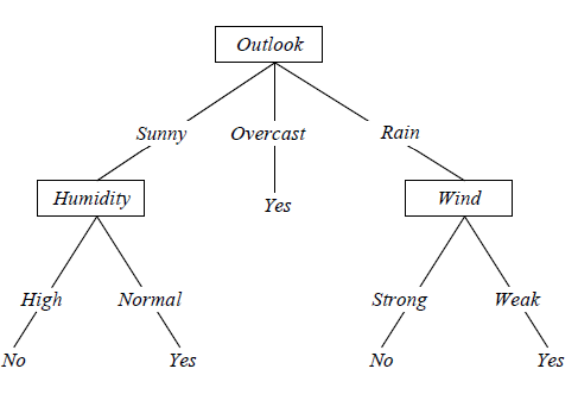
\includegraphics[width=0.5\textwidth]{dt-diagram.png}}
		\caption{درخت تصمیم}
		\label{fig}
	\end{figure}
	
	
	\subsection*{توضیحات تکمیلی}
	\begin{itemize}
		\item [$\bullet$] انجام پروژه می‌تواند در قالب گروه های دو نفره و یا به صورت انفرادی صورت گیرد.
		
		\item [$\bullet$] علاوه بر سورس کد پروژه، فایل مستندات  نیز باید آپلود شود.
		
		\item [$\bullet$] در فایل مستندات پروژه نام هر دو عضو گروه را ذکر کنید و آپلود فایل‌ها همین که توسط یکی از اعضای گروه انجام شود کافی است.
		
		\item [$\bullet$] هر گونه شباهت نامتعارف بین کد شما و کد سایر گروه‌ها و یا کدها‌ی موجود بر روی اینترنت تقلب محسوب می‌شود و نمره‌ای برای این پروژه دریافت نخواهید کرد.
		
		\item [$\bullet$] در صورت نوشتن داکیومنت تمیز (برای مثال با \lr{\LaTeX}) نمره اضافه برای شما در نظر گرفته خواهد شد.
		
		\item [$\bullet$] استفاده از هرگونه روش خلاقانه نمره اضافی خواهد داشت.
		
		\item [$\bullet$] استفاده از کتابخانه ها و فریم ورک‌های آماده به جز مواردی که درصورت پروژه از شما خواسته شده تا پیاده سازی کنید، بلامانع است.
		
		\item [$\bullet$] فایل شامل سورس کد پروژه و مستندات را در قالب فایل \lr{zip} و با نام شماره دانشجویی خود ذخیره و ارسال نمائید.
		
		\item [$\bullet$] در صورت داشتن هرگونه سوال می‌توانید با \lr{\href{https://t.me/kourosh_hsz}{\textcolor{blue}{\lr{kourosh\_hsz}}}} و یا \lr{\href{https://t.me/mhmdrzrs}{\textcolor{blue}{\lr{mhmdrzrs}}}} در ارتباط باشید و یا در گروه درسی مطرح نمائید.
		\newline
	\end{itemize}
	
	\begin{LTR}
		
		تمرین حل تیم - احترام با
	\end{LTR}
	
	
	
\end{document}
